\documentclass[a4paper, amsfonts, amssymb, amsmath, reprint, showkeys, nofootinbib, twoside]{revtex4-1}
\usepackage[english]{babel}
\usepackage[utf8]{inputenc}
\usepackage[colorinlistoftodos, color=green!40, prependcaption]{todonotes}
\usepackage[pdftex, pdftitle={Article}, pdfauthor={Author}]{hyperref}
\usepackage{amsthm}
\usepackage{mathtools}
\usepackage{physics}
\usepackage{xcolor}
\usepackage{caption}
\usepackage{hyperref}
\usepackage{multirow}
\usepackage{amsmath}
\usepackage{amssymb}
\usepackage{graphicx}
\graphicspath{Images}
\usepackage[left=23mm,right=13mm,top=35mm,columnsep=15pt]{geometry} 
\usepackage{adjustbox}
\usepackage{placeins}
\usepackage[T1]{fontenc}
\usepackage{float}
%\usepackage{longtable}
\usepackage{csquotes}
\usepackage{refstyle}
\usepackage{lipsum}
\usepackage{booktabs}

\begin{document}

\title{Applications of Geiger-Muller Counter}
\author{Swaroop Ramakant Avarsekar}
\email{swaroop.avarsekar@niser.ac.in}
\affiliation{School of Physical Sciences, National Institute of Science Education and Research, HBNI, Jatni -752050, India}
\date{\today}

\begin{abstract}
We study the range and back scattering of beta particles, production and attenuation of Bremsstrahlung as part of application of GM counter. Tl-204 and Sr-90 is used as beta sources. The range of beta particles for Sr-90 was found to be $0.711g/cm^2$ and end point energy as 1.54 MeV. In back scattering, the saturation thickness could not be estimated. In Bremsstrahlung, the count rate of perspex was lower than metals and the rate was comparable between Al and Cu. Also short half life of radioactive sample is also calculated. Mixture of 0.9\% NaCl in 0.04 M HCl as used as a solvent which is mixed with Cs-137 isotope generator. Half life of the same was found to be 385.726$\pm$ 3.434 s. 
\end{abstract}
	
\keywords{Bremsstrahlung, End point energy, Back-scattering}
\maketitle
\section{Theory}
\subsection{Range of Beta Particles }
A widely used empirical formula for the range of beta particles related to its end point energy in the Aluminum absorber is given by,
\begin{equation}
	R=(0.52E-0.09) g/cm^2
\end{equation}
where E is end point energy of beta source. 

To calculate range by half thickness method, we have,
\begin{equation}
\frac{t_1^{1/2}}{t_2^{1/2}}=R_1/R_2
\end{equation}
where  $t_1^{1/2}$ and $t_2^{1/2}$ are thickness of Al at half count rate for two sources and $R_1$ and $R_2$ are range of $\beta$ particles from two sources.

We use Tl-204 and Sr-90 as source for experiment.

\subsection{Back-Scattering of Beta Particles}


Absorption occur when collision of beta particles with matter, scattering may also occur due to collision with increasing atomic no. Back scattering occurs when angle of deflection is greater than 90$^\circ$, which is dependent on material. Higher atomic no. scattering occurs at large angle with little loss of energy. Back scattering is proportional to $\sqrt{Z}$. Thickness of material influence Back scattering upto a saturation point with maximum value attaining thickness less than range of beta particles. 



\subsection{Bremsstrahlung}
Bremsstrahlung is electromagnetic radiation produced by deceleration of charged particles like electron. It looses kinetic energy and converted to a photon. Bremsstrahlung has continuous spectrum becomes intense as intensity shifts towards higher frequencies. the intensity increases with the atomic no./density goes up. If the mass per unit area of plates used as absorbers such that beta particles are completely absorbed, then materials with higher atomic density, higher Bremsstrahlung count rate is obtained.
\section{Experiment and Analysis}
\subsection{Range of Beta Particles }
\begin{table}[H]
	\centering
	\caption{Background count}
	\label{t1}
		\begin{tabular}{|r|r|}
			\hline
			\multicolumn{1}{|l|}{Sl no.}  & \multicolumn{1}{l|}{Count} \\ \hline
			1                             & 62                         \\ \hline
			2                             & 51                         \\ \hline
			3                             & 54                         \\ \hline
			4                             & 58                         \\ \hline
			5                             & 55                         \\ \hline
			\multicolumn{1}{|l|}{Average} & \multicolumn{1}{l|}{56}    \\ \hline
		\end{tabular}
\end{table}

\begin{table}[H]
	\centering
	\caption{Source:Tl-204, Absorber: Al}
	\label{t2}
	\resizebox{\columnwidth}{!}{%
		\begin{tabular}{|c|c|c|c|}
			\hline
			\begin{tabular}[c]{@{}c@{}}Absorber \\ Thickness (mm)\end{tabular} &
			\begin{tabular}[c]{@{}c@{}}Absorber Thickness\\  (mg/$cm^2$)\end{tabular} &
			Counts &
			\begin{tabular}[c]{@{}c@{}}Net \\ Counts\end{tabular} \\ \hline
			0    & 0      & 12653 & 12597 \\ \hline
			0.06 & 16.26  & 9120  & 9064  \\ \hline
			0.12 & 32.52  & 6776  & 6720  \\ \hline
			0.18 & 48.78  & 5262  & 5206  \\ \hline
			0.24 & 65.04  & 3834  & 3778  \\ \hline
			0.3  & 81.3   & 2206  & 2150  \\ \hline
			0.36 & 97.56  & 2015  & 1959  \\ \hline
			0.42 & 113.82 & 1188  & 1132  \\ \hline
			0.48 & 130.08 & 1206  & 1150  \\ \hline
			0.54 & 146.34 & 864   & 808   \\ \hline
		\end{tabular}%
	}
\end{table}

\begin{table}[H]
	\centering
	\caption{Source:Sr-90, Absorber: Al}
	\label{t3}
	\resizebox{\columnwidth}{!}{%
		\begin{tabular}{|c|c|c|c|}
			\hline
			\begin{tabular}[c]{@{}c@{}}Absorber \\ Thickness (mm)\end{tabular} &
			\begin{tabular}[c]{@{}c@{}}Absorber Thickness\\  (mg/$cm^2$)\end{tabular} &
			Counts &
			\begin{tabular}[c]{@{}c@{}}Net \\ Counts\end{tabular} \\ \hline
			0    & 0      & 10088 & 10033 \\ \hline
			0.06 & 16.26  & 8074  & 8019  \\ \hline
			0.12 & 32.52  & 7315  & 7260  \\ \hline
			0.18 & 48.78  & 6247  & 6192  \\ \hline
			0.24 & 65.04  & 5684  & 5629  \\ \hline
			0.3  & 81.3   & 5273  & 5218  \\ \hline
			0.36 & 97.56  & 4814  & 4759  \\ \hline
			0.42 & 113.82 & 4440  & 4385  \\ \hline
			0.48 & 130.08 & 4173  & 4118  \\ \hline
			0.54 & 146.34 & 4119  & 4064  \\ \hline
		\end{tabular}%
	}
\end{table}

\begin{figure}[H]
	\centering
	\includegraphics[scale=0.6]{1tl} 
	\caption{Net Count vs Thickness curve for Tl-204}
	\label{1}
\end{figure}

\begin{figure}[H]
	\centering
	\includegraphics[scale=0.6]{2sr} 
	\caption{Net Count vs Thickness curve for Sr-90}
	\label{2}
\end{figure}

We obtain thickness of Al required to reduce the count rate by half is $t_1^{1/2}\approx38~gm/cm^2$ and $t_2^{1/2}\approx~88gm/cm^2$ where $t_1^{1/2}$ is thickness of Al for Tl-204 and Sr-90, respectively.

The end point energy of Tl-204 is 0.764 MeV. Therefore, Range of beta particles from Tl-204 is 
\begin{equation}
	R_1=(0.52E_o-0.09)
\end{equation}

\begin{equation}
	R_1=(0.52\times0.764-0.09)=0.30728 g/cm^2
\end{equation}

Therefore,
\begin{equation}
	\frac{t_1^{1/2}}{t_2^{1/2}}=\frac{R_1}{R_2}
\end{equation}

\begin{equation}
	\frac{t_2^{1/2}}{t_1^{1/2}}\times R_1=R_2
\end{equation}

\begin{equation}
	R_2=\frac{88}{38}\times 0.30728 ~g/cm^2=0.711~g/cm^2
\end{equation}

End-point energy of Sr-90 is
\begin{equation}
	E_2=\frac{R_2+0.09}{0.52}
\end{equation}

\begin{equation}
	E_2=\frac{0.711+0.09}{0.52}=1.54 MeV
\end{equation}

\subsection{Back-Scattering of Beta Particles}
\begin{table}[H]
	\centering
	\caption{Material-Al, Preset time-200 s}
	\label{t4}
		\begin{tabular}{|c|ccc|c|}
			\hline
			\multirow{2}{*}{\begin{tabular}[c]{@{}c@{}}Thickness\\  (mm)\end{tabular}} &
			\multicolumn{3}{c|}{Counts} &
			\multirow{2}{*}{\begin{tabular}[c]{@{}c@{}}Net\\  Counts\end{tabular}} \\ \cline{2-4}
			& \multicolumn{1}{c|}{I}   & \multicolumn{1}{c|}{II}  & Avg   &      \\ \hline
			0    & \multicolumn{1}{c|}{208} & \multicolumn{1}{c|}{182} & 195   & -    \\ \hline
			0.05 & \multicolumn{1}{c|}{217} & \multicolumn{1}{c|}{194} & 205.5 & 10.5 \\ \hline
			0.1  & \multicolumn{1}{c|}{205} & \multicolumn{1}{c|}{222} & 213.5 & 18.5 \\ \hline
			0.15 & \multicolumn{1}{c|}{208} & \multicolumn{1}{c|}{202} & 205   & 10   \\ \hline
			0.2  & \multicolumn{1}{c|}{197} & \multicolumn{1}{c|}{213} & 205   & 10   \\ \hline
			0.25 & \multicolumn{1}{c|}{233} & \multicolumn{1}{c|}{221} & 227   & 32   \\ \hline
			0.3  & \multicolumn{1}{c|}{226} & \multicolumn{1}{c|}{225} & 225.5 & 30.5 \\ \hline
			0.35 & \multicolumn{1}{c|}{208} & \multicolumn{1}{c|}{210} & 209   & 14   \\ \hline
			0.4  & \multicolumn{1}{c|}{215} & \multicolumn{1}{c|}{241} & 228   & 33   \\ \hline
			0.45 & \multicolumn{1}{c|}{196} & \multicolumn{1}{c|}{180} & 188   & -7   \\ \hline
			0.5  & \multicolumn{1}{c|}{162} & \multicolumn{1}{c|}{192} & 177   & -18  \\ \hline
			0.55 & \multicolumn{1}{c|}{210} & \multicolumn{1}{c|}{184} & 197   & 2    \\ \hline
			0.6  & \multicolumn{1}{c|}{198} & \multicolumn{1}{c|}{202} & 200   & 5    \\ \hline
			0.65 & \multicolumn{1}{c|}{200} & \multicolumn{1}{c|}{181} & 190.5 & -4.5 \\ \hline
		\end{tabular}
\end{table}

\begin{figure}[H]
	\centering
	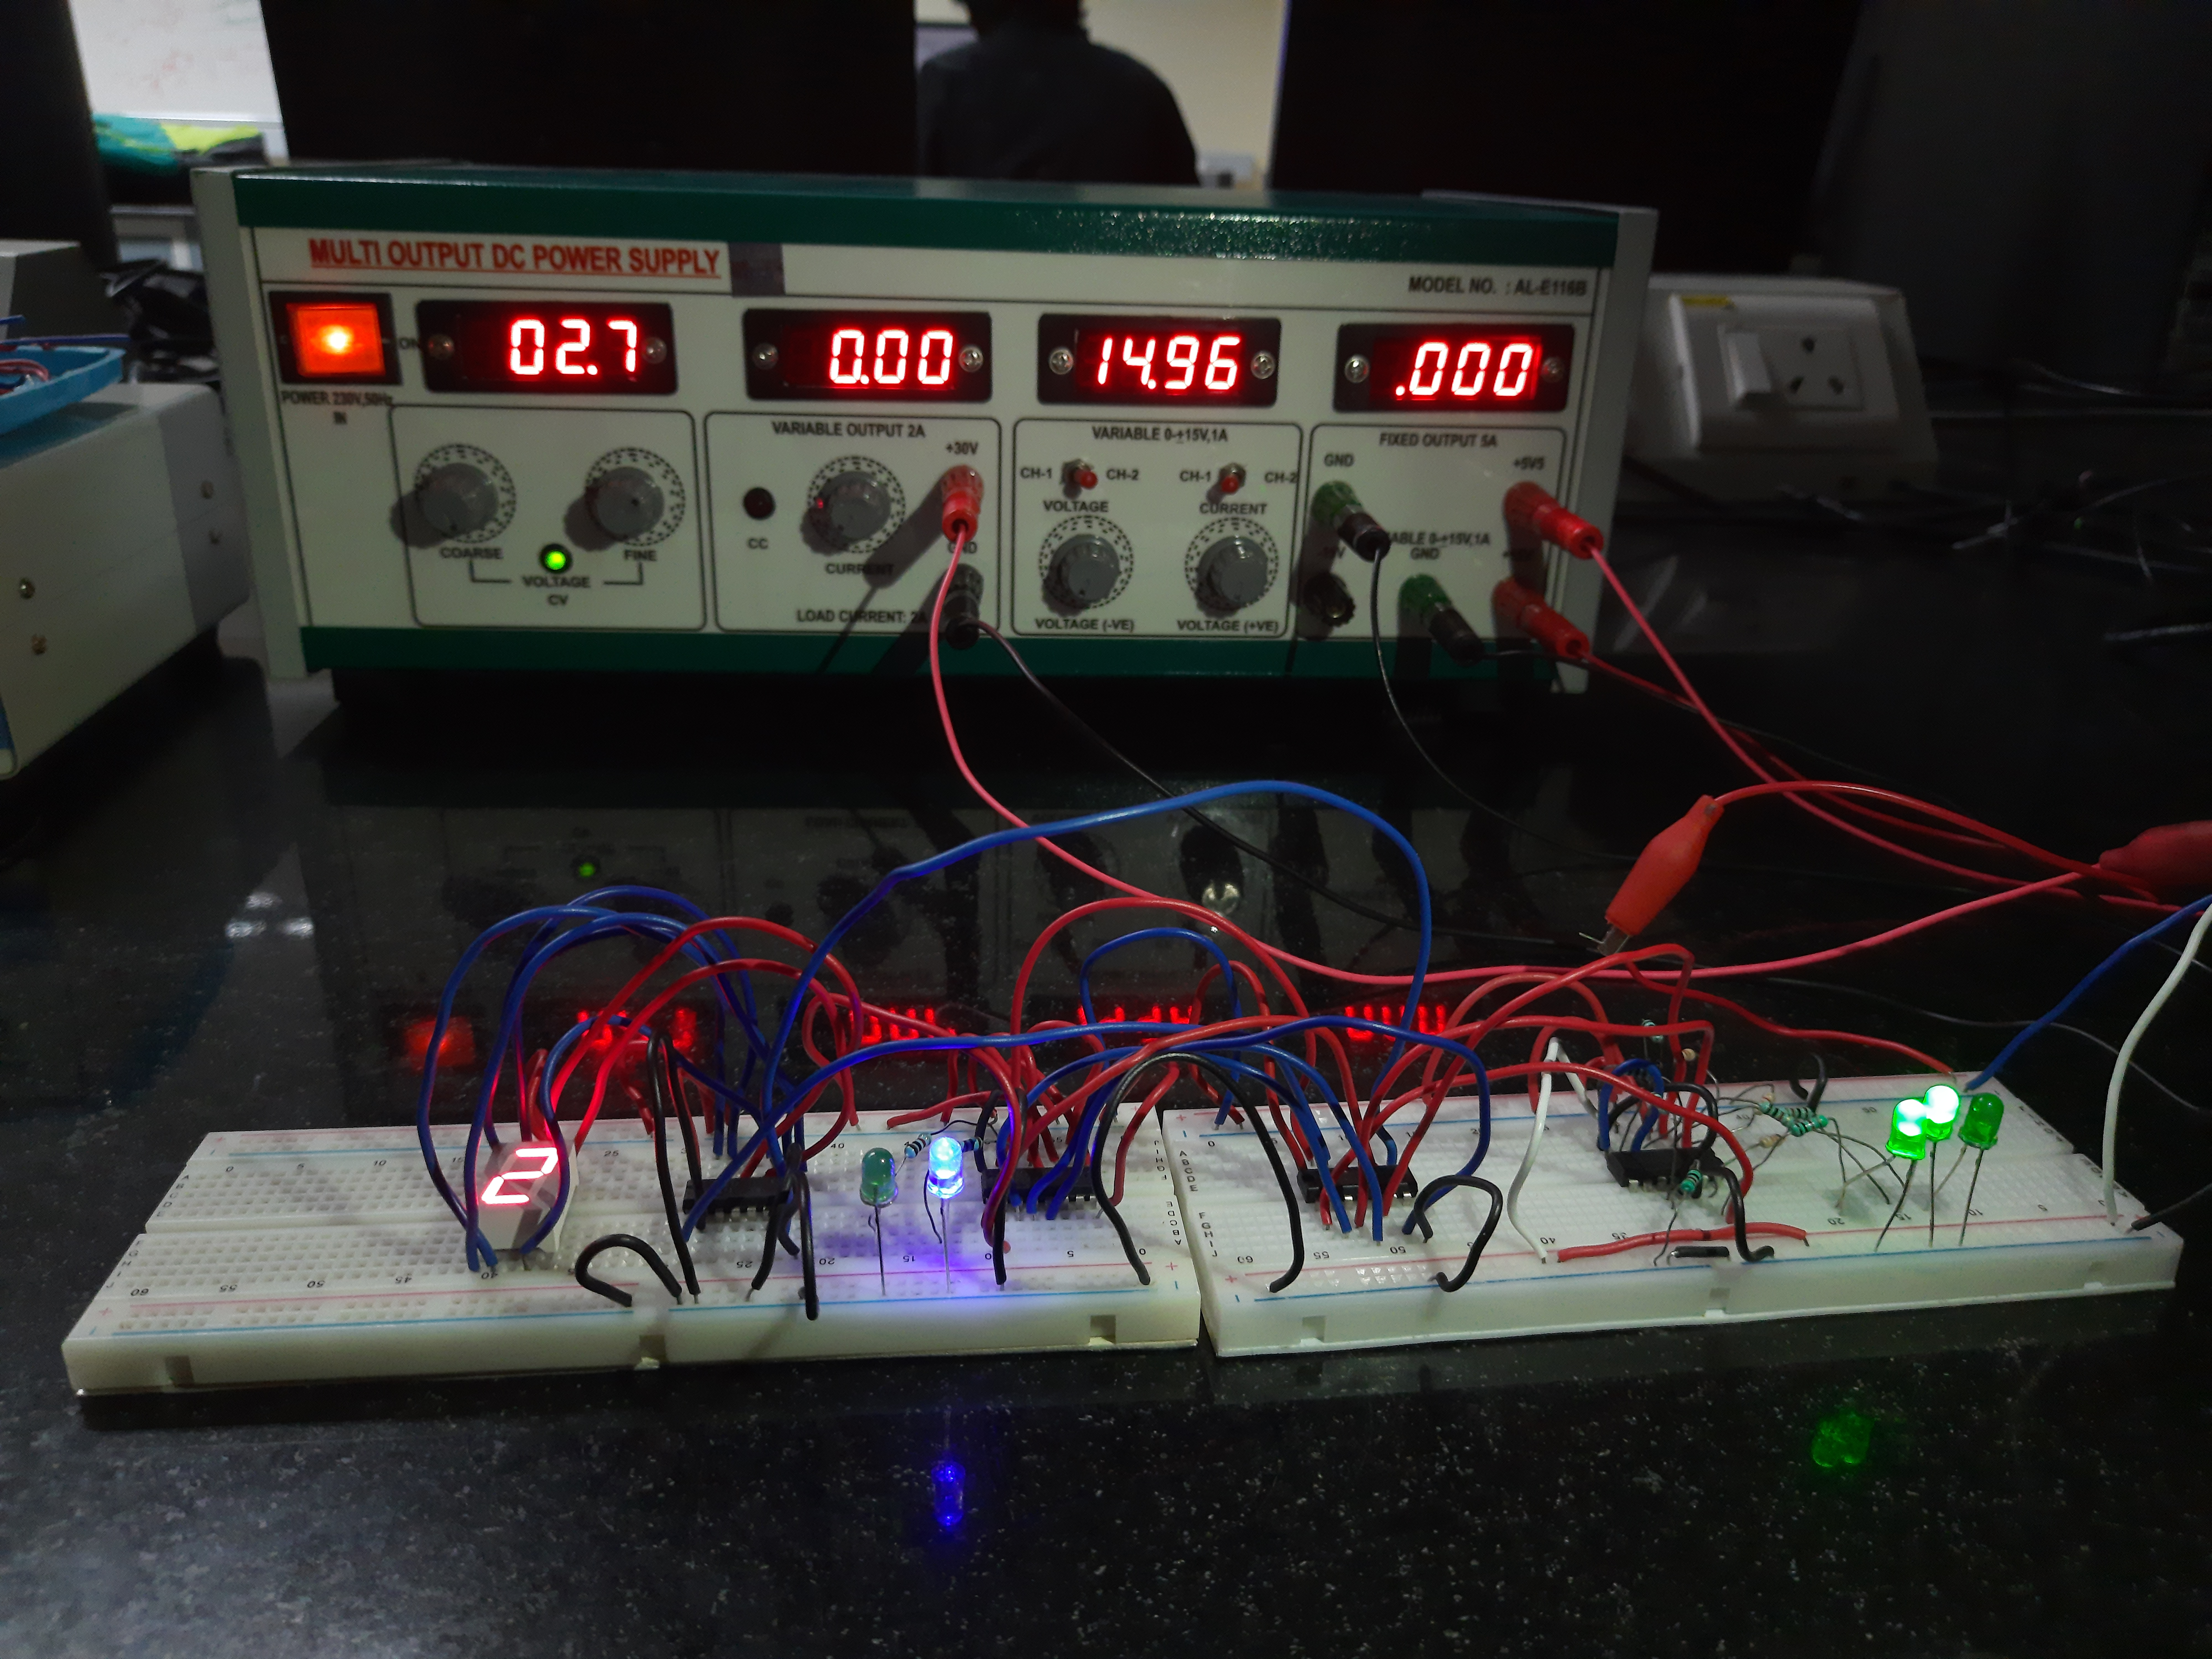
\includegraphics[scale=0.4]{2} 
	\caption{Net Count vs Thickness curve for Back scattering}
	\label{3}
\end{figure}

The angle between source and detector was set to 100$^\circ$. It was expected to be saturated but counts was not read as expected. It may happened due to usage of source on two different days may have resulted in unexpected count as experiment was done on two different days. Therefore, this experiment failed to determine saturation thickness of the material.
\subsection{Bremsstrahlung}


Sr-90 source was used with preset time of 300s and distance between source and detector as 6 cm and activity of 0.1 mCi. The Background count is 307.
The observation of Bremsstrahlung is shown in tables V, VI and VII.

\begin{table}[H]
	\centering
	\caption{For Al(0.7 mm) and Perspex (1.8 mm) combination}
	\label{t5}
	\resizebox{\columnwidth}{!}{%
		\begin{tabular}{|c|c|c|c|}
			\hline
			S. No. & Absorber Position     & Counts & Net Counts \\ \hline
			1      & -                     & 6812   & 6505       \\ \hline
			2      & Perspex facing source & 395    & 88         \\ \hline
			3      & Al. facing Source     & 495    & 188        \\ \hline
		\end{tabular}%
	}
\end{table} 

\begin{table}[H]
	\centering
	\caption{For  Perspex (1.8 mm) and Cu(0.3mm) combination}
	\label{t6}
	\resizebox{\columnwidth}{!}{%
		\begin{tabular}{|c|c|c|c|}
			\hline
			S. No. & Absorber Position    & Counts & Net Counts \\ \hline
			1      & -                    & 7554   & 7247       \\ \hline
			2      & Perspex facing source     & 434    & 127        \\ \hline
			3      & Cu facing Source & 445    & 138        \\ \hline
		\end{tabular}%
	}
\end{table}

\begin{table}[H]
	\centering
	\caption{For  Al (1.8 mm) and Cu(0.3mm) combination}
	\label{t7}
	\resizebox{\columnwidth}{!}{%
		\begin{tabular}{|c|c|c|c|}
			\hline
			S. No. & Absorber Position & Counts & Net Counts \\ \hline
			1      & -                 & 7562   & 7255       \\ \hline
			2      & Cu facing source  & 414    & 107        \\ \hline
			3      & Al facing Source  & 410    & 103        \\ \hline
		\end{tabular}%
	}
\end{table}

The count rate of Bremsstrahlung depends on order of arrangement of the materials. We can see from table V that the count rate for the perspex is low with that of aluminium, since Bremsstrahlung generated is not absorbed in metals. Even for perspex-Cu combination, shown in table VI, we see count rate of Cu is higher than perspex. With the combination of Al-Cu, as shown in table VII, the count rate is almost similar in both the materials.


\subsection{Short half life}
A mixture of 0.9\% NaCl in 0.04 M HCl is used as a solvent which is mixed with Cs-137 isotope generator. The mixture is used to take the count reading. The background count was found to be 294. 

\begin{figure}[H]
	\centering
	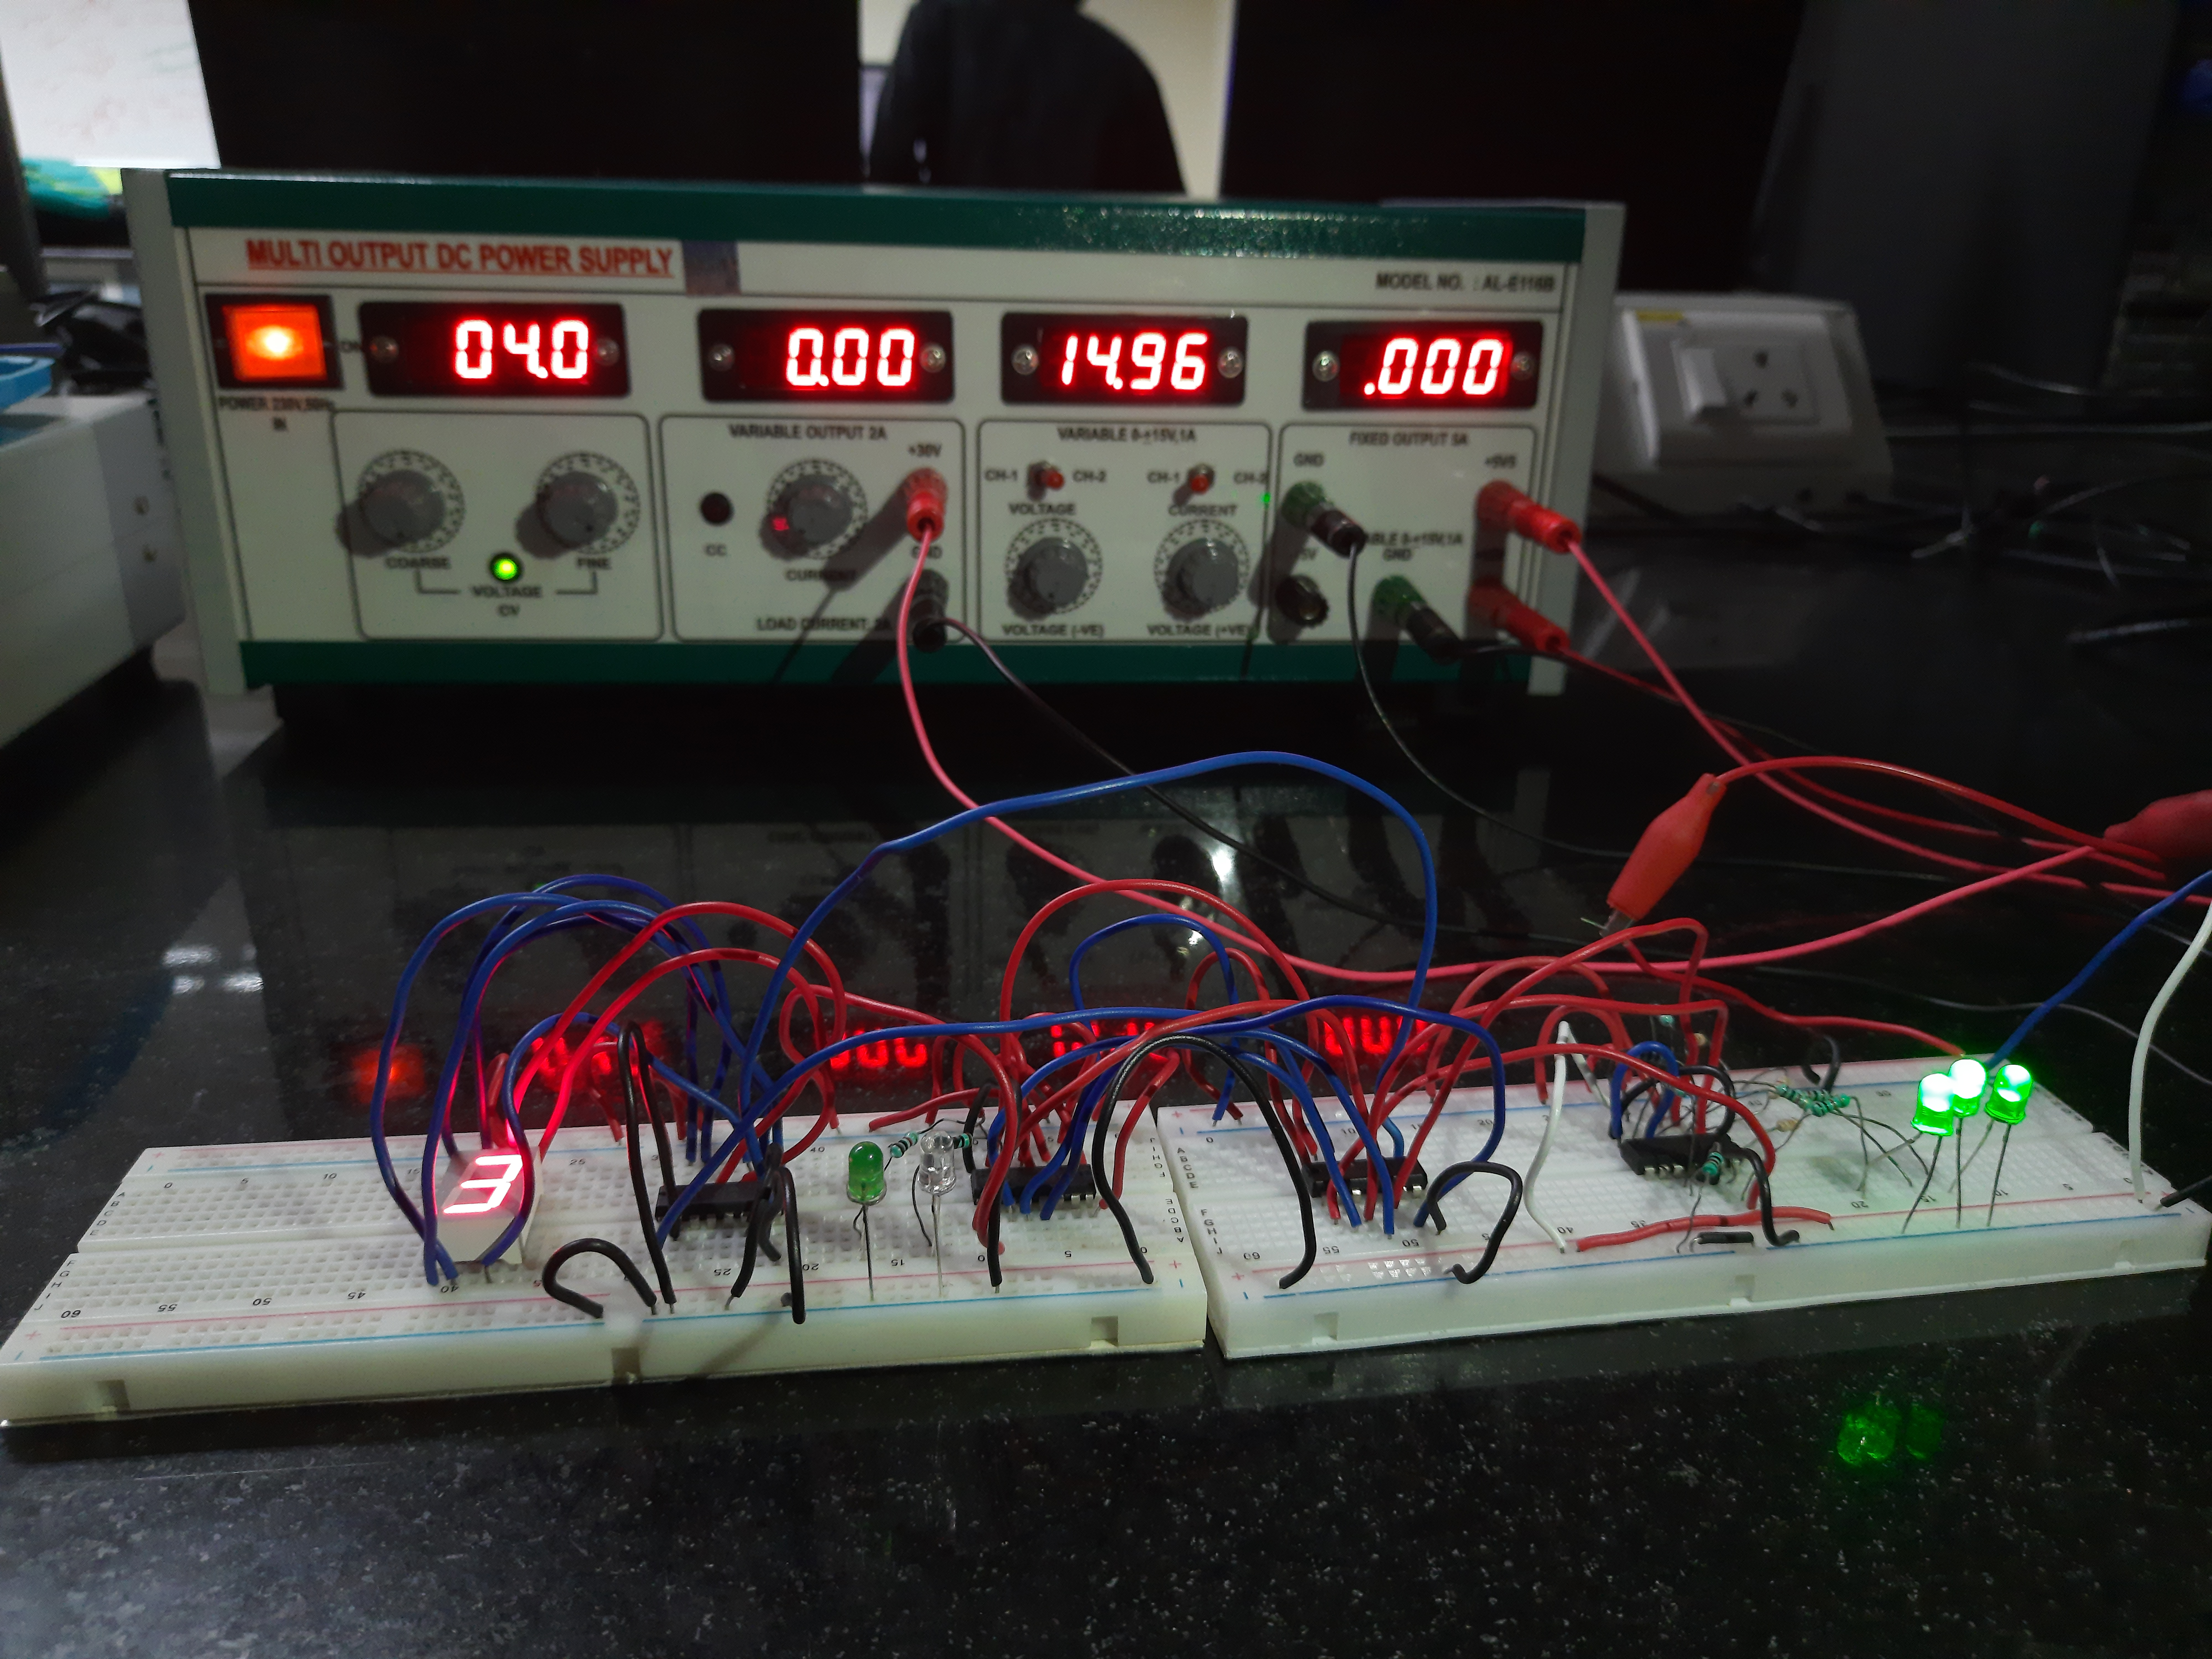
\includegraphics[scale=0.09]{3} 
	\caption{Solvent used for generator}
\end{figure}

\begin{figure}[H]
	\centering
	\includegraphics[scale=0.06]{4} 
	\caption{Cs-137 Isotope generator.}
\end{figure}

\begin{figure}[H]
	\centering
	\includegraphics[scale=0.6]{lnt} 
	\caption{Plot of ln(N) versus time}
\end{figure}

\begin{table}[H]
	\centering
	\caption{Determination of short half life}
	\label{t8}
	\resizebox{\columnwidth}{!}{%
		\begin{tabular}{|c|c|c|c|c|}
			\hline
			S. No. & \begin{tabular}[c]{@{}c@{}}Elapsed \\ Time (s)\end{tabular} & Counts & \begin{tabular}[c]{@{}c@{}}Corrected \\ count/s\end{tabular} & ln(N) \\ \hline
			1  & 20  & 3840  & 177.30 & 5.177843213 \\ \hline
			2  & 30  & 5592  & 176.60 & 5.173887288 \\ \hline
			3  & 40  & 7337  & 176.08 & 5.170910041 \\ \hline
			4  & 50  & 8904  & 172.20 & 5.148656592 \\ \hline
			5  & 60  & 10519 & 170.42 & 5.138246419 \\ \hline
			6  & 70  & 12019 & 167.50 & 5.120983351 \\ \hline
			7  & 80  & 13485 & 164.89 & 5.105263423 \\ \hline
			8  & 90  & 14815 & 161.34 & 5.083541486 \\ \hline
			9  & 100 & 16059 & 157.65 & 5.060377386 \\ \hline
			10 & 110 & 17262 & 154.25 & 5.03860413  \\ \hline
			11 & 120 & 18425 & 151.09 & 5.017886717 \\ \hline
			12 & 130 & 19600 & 148.51 & 5.000636757 \\ \hline
			13 & 140 & 20674 & 145.57 & 4.980666884 \\ \hline
			14 & 150 & 21718 & 142.83 & 4.961631774 \\ \hline
			15 & 160 & 22742 & 140.30 & 4.943782987 \\ \hline
			16 & 170 & 23786 & 138.19 & 4.92861678  \\ \hline
			17 & 180 & 24648 & 135.30 & 4.907494535 \\ \hline
			18 & 190 & 25559 & 132.97 & 4.890151246 \\ \hline
			19 & 200 & 26401 & 130.54 & 4.87164139  \\ \hline
			20 & 210 & 27229 & 128.26 & 4.854074304 \\ \hline
			21 & 220 & 28040 & 126.12 & 4.837219418 \\ \hline
			22 & 230 & 28808 & 123.97 & 4.820071165 \\ \hline
			23 & 240 & 29526 & 121.80 & 4.802380355 \\ \hline
			24 & 250 & 30240 & 119.78 & 4.785690121 \\ \hline
			25 & 260 & 30896 & 117.70 & 4.768139014 \\ \hline
			26 & 270 & 31557 & 115.79 & 4.75176861  \\ \hline
			27 & 280 & 32185 & 113.90 & 4.735289514 \\ \hline
			28 & 290 & 32799 & 112.09 & 4.71926828  \\ \hline
			29 & 300 & 33392 & 110.33 & 4.703445662 \\ \hline
		\end{tabular}%
}
\end{table}

We have slope as -0.001797 $\pm$ 0.000016 $s^{-1}$ with intercept as 5.238$\pm$ 0.002. The intercept gives as initial count, ln(N)=5.238 implying 188.29 count/s. Therefore, decay constant is the slope, $\lambda=-0.001797 s^{-1}$. Hence,
\begin{equation}
	t_{1/2}=0.693/\lambda=385.726 s
\end{equation}

Error in $t_{1/2}$ is given by:
\begin{equation}
	\delta t_{1/2}=t_{1/2}\times \delta \lambda/\lambda
\end{equation}

\begin{equation}
	\delta t_{1/2}=385.726\times 0.000016/0.001797=3.434s
\end{equation}

The short half life of the mixture is 385.726$\pm$ 3.434 s, with initial count as 188.29 count/s.

\section{Conclusion}
We studied the range of beta particles and calculated the end point energy of Sr-90. The other source was Tl-204 used as reference. We determined the range as $0.711 g/cm^2$ by half thickness method and end point energy as 1.54 MeV. Backscattering with Al as absorber was also studied. In this part of experiment, we were unable to determine the saturation thickness as experiment have been performed in two different days. The Bremsstrahlung was studied and the count rate was expected based on the order of the materials. Combination of Al, Cu and Perspex was used. It was seen that count rate is low for perspex as 188.29 count/s. Bremsstrahlung generated is not absorbed for Al and Cu. The count rate of Al and Cu was comparable. We also determined the half life of mixture of 0.9\% NaCl in 0.04 M HCl as used as a solvent which is mixed with Cs-137 isotope generator. It was found to be 385.726$\pm$ 3.434 s with initial count as 

One of the ways to improve the back scattering experiment to get thickness saturation is by setting angle between the source and detector to optimal obtuse angle based on several trials and marking the positions of the source and detector.  Good aluminium sheets must be used for this experiment. Torn sheets may give inaccurate count readings. It is to be noted that they should be blocked by lead block. Also the count rate is not continuous and exact in the GM counter as it can only count upto a limited number. One must take precautionary measure while handling
radioactive sources.

\section{References}
\begin{enumerate}
\item{\url{NISER lab manual}}
%\item{\url{}}
\end{enumerate}

\end{document}